%%%%%%%%%%%%%%%%%%%%%%%%%%%%%%%%%%%%%%%%%%%%%%%%%%%%%%%%%%%%%%%%%%%%%%
%     File: ExtendedAbstract_imple.tex                               %
%     Tex Master: ExtendedAbstract.tex                               %
%                                                                    %
%     Author: Andre Calado Marta                                     %
%     Last modified : 27 Dez 2011                                    %
%%%%%%%%%%%%%%%%%%%%%%%%%%%%%%%%%%%%%%%%%%%%%%%%%%%%%%%%%%%%%%%%%%%%%%
% A Calculation section represents a practical development
% from a theoretical basis.
%%%%%%%%%%%%%%%%%%%%%%%%%%%%%%%%%%%%%%%%%%%%%%%%%%%%%%%%%%%%%%%%%%%%%%

\section{Implementation}
\label{sec:imple}

Our comparison with the auxiliary field QMC results of \texttt{QUEST} for a 64-site system with $U = 4 t$, and $beta = 25 t$, show  remarkable agreement.
\begin{figure}[H]
  \centering
  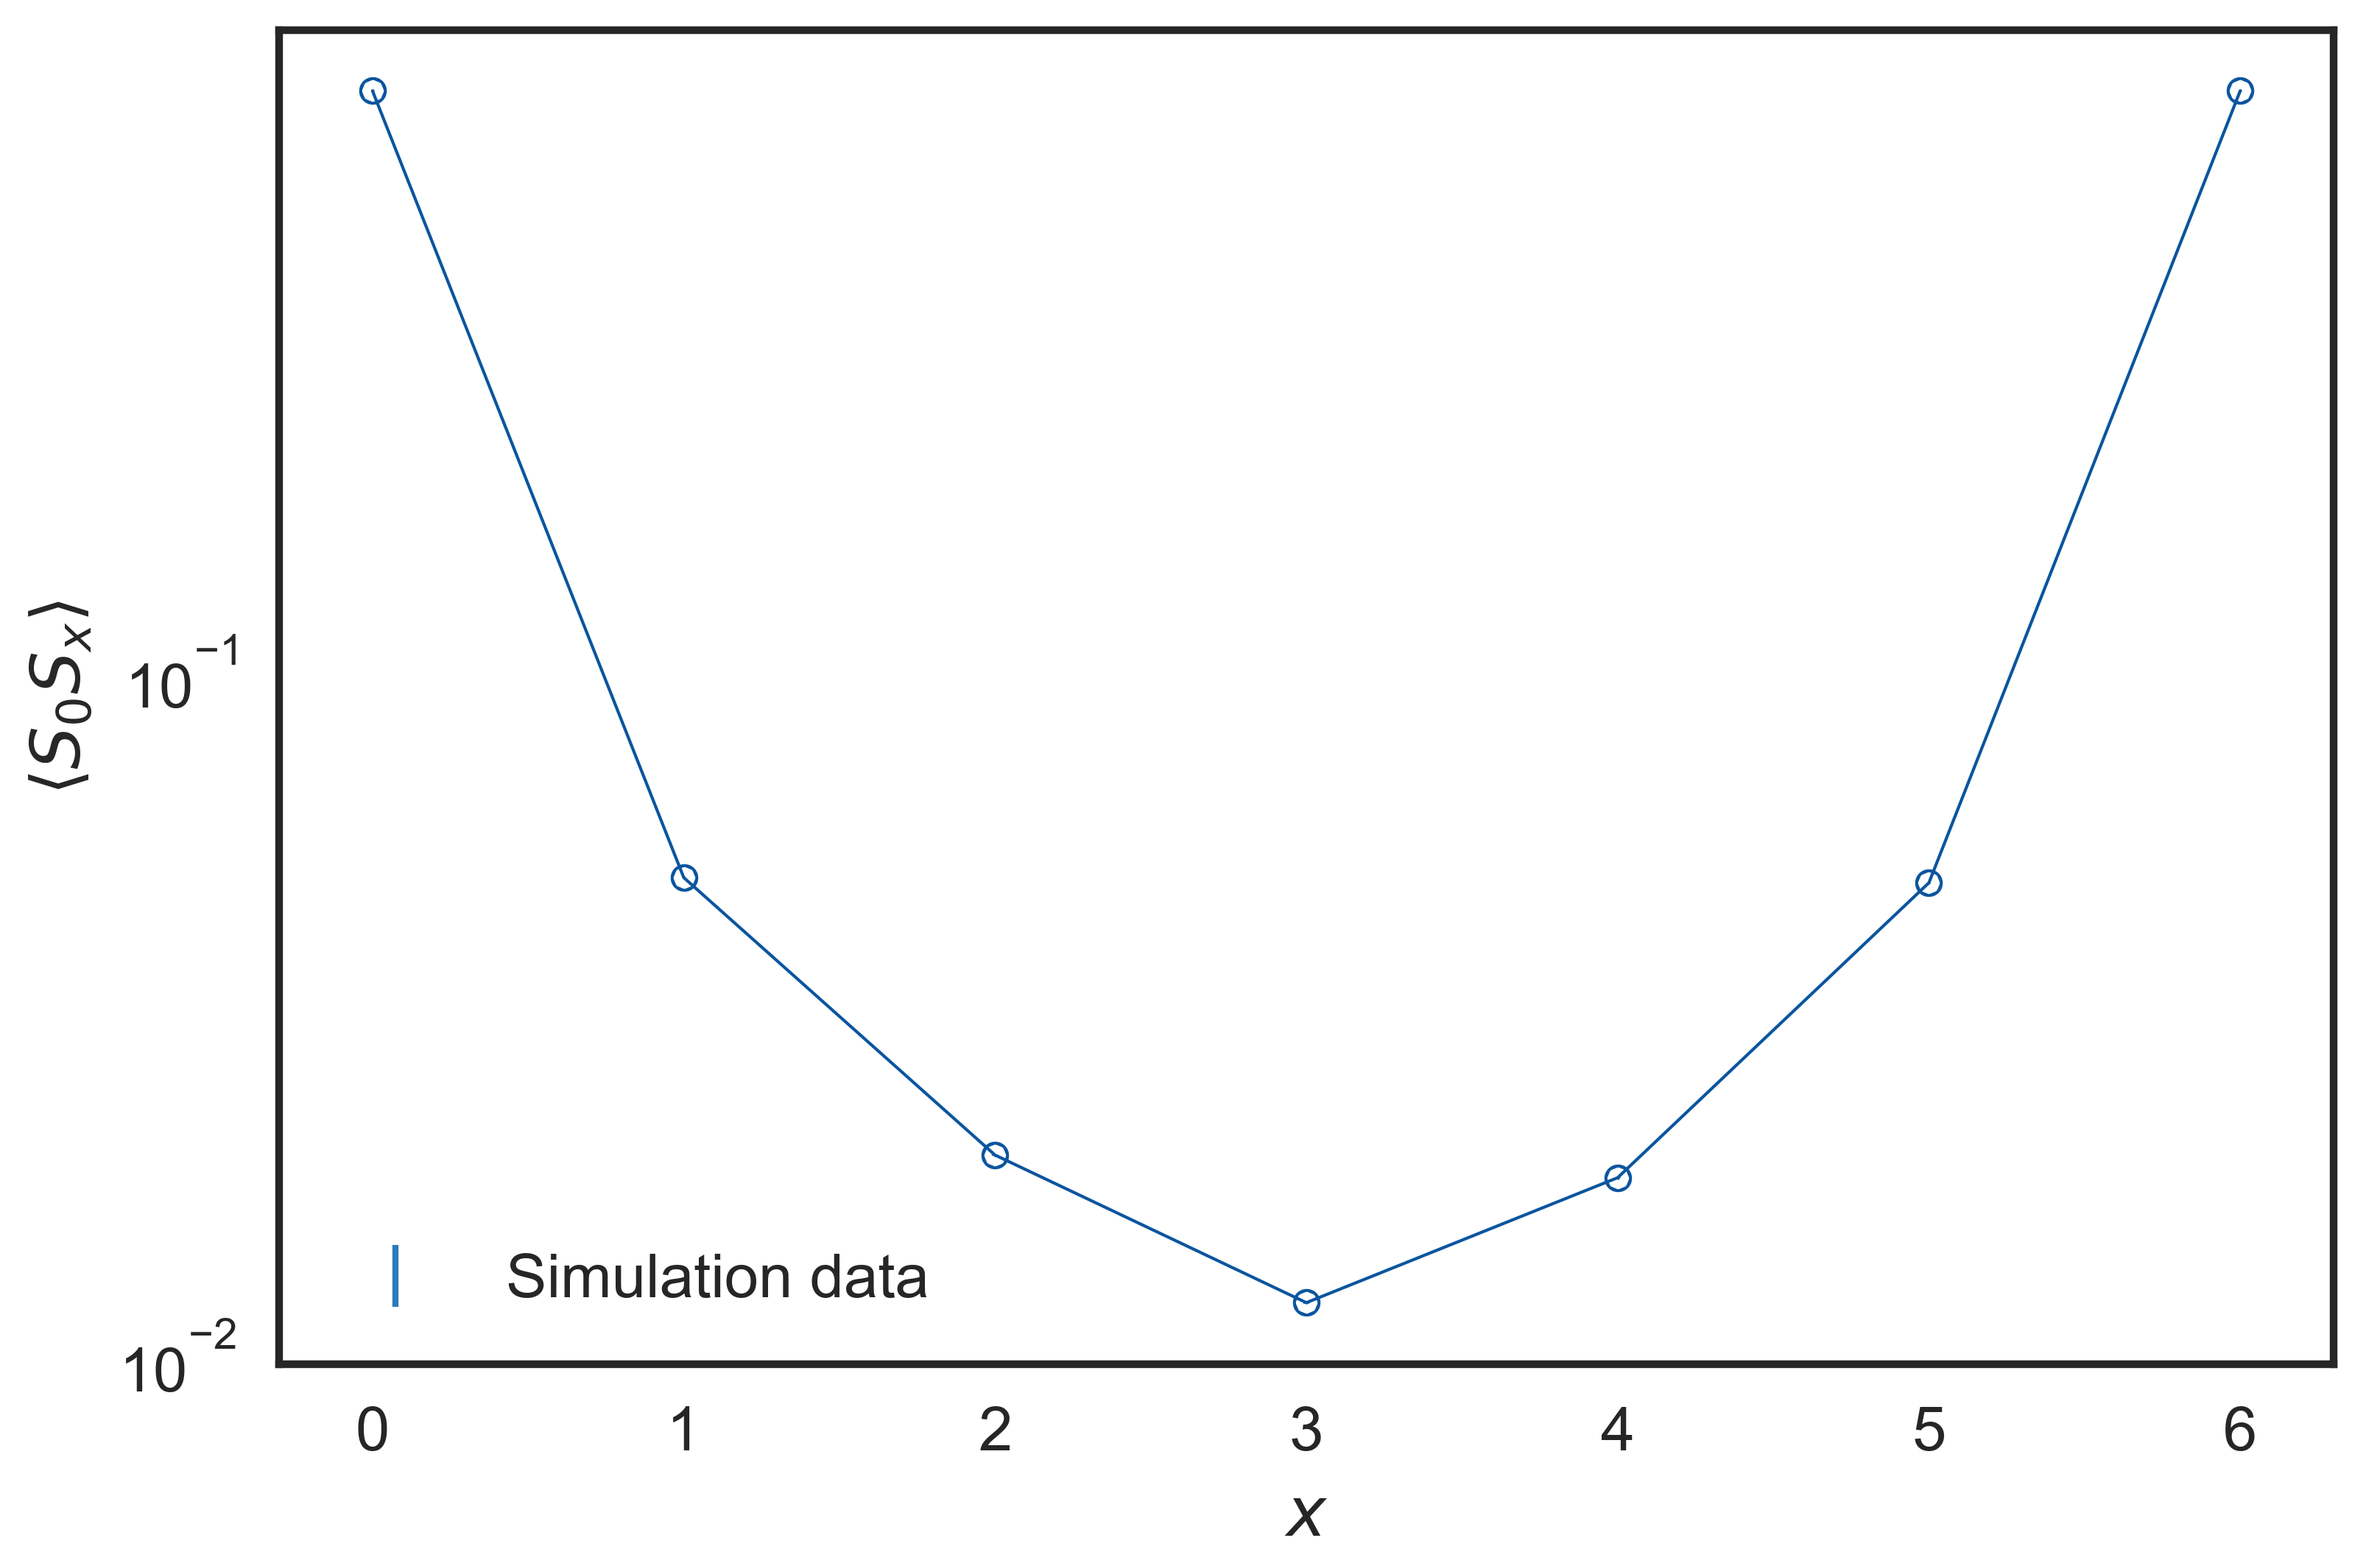
\includegraphics[width=6cm]{images/LongitudinalProfile.png}
  \caption{Comparison with \texttt{QUEST}}
  \label{fig:blade_flow_pressure}
\end{figure}

\begin{figure}[H]
  \centering
  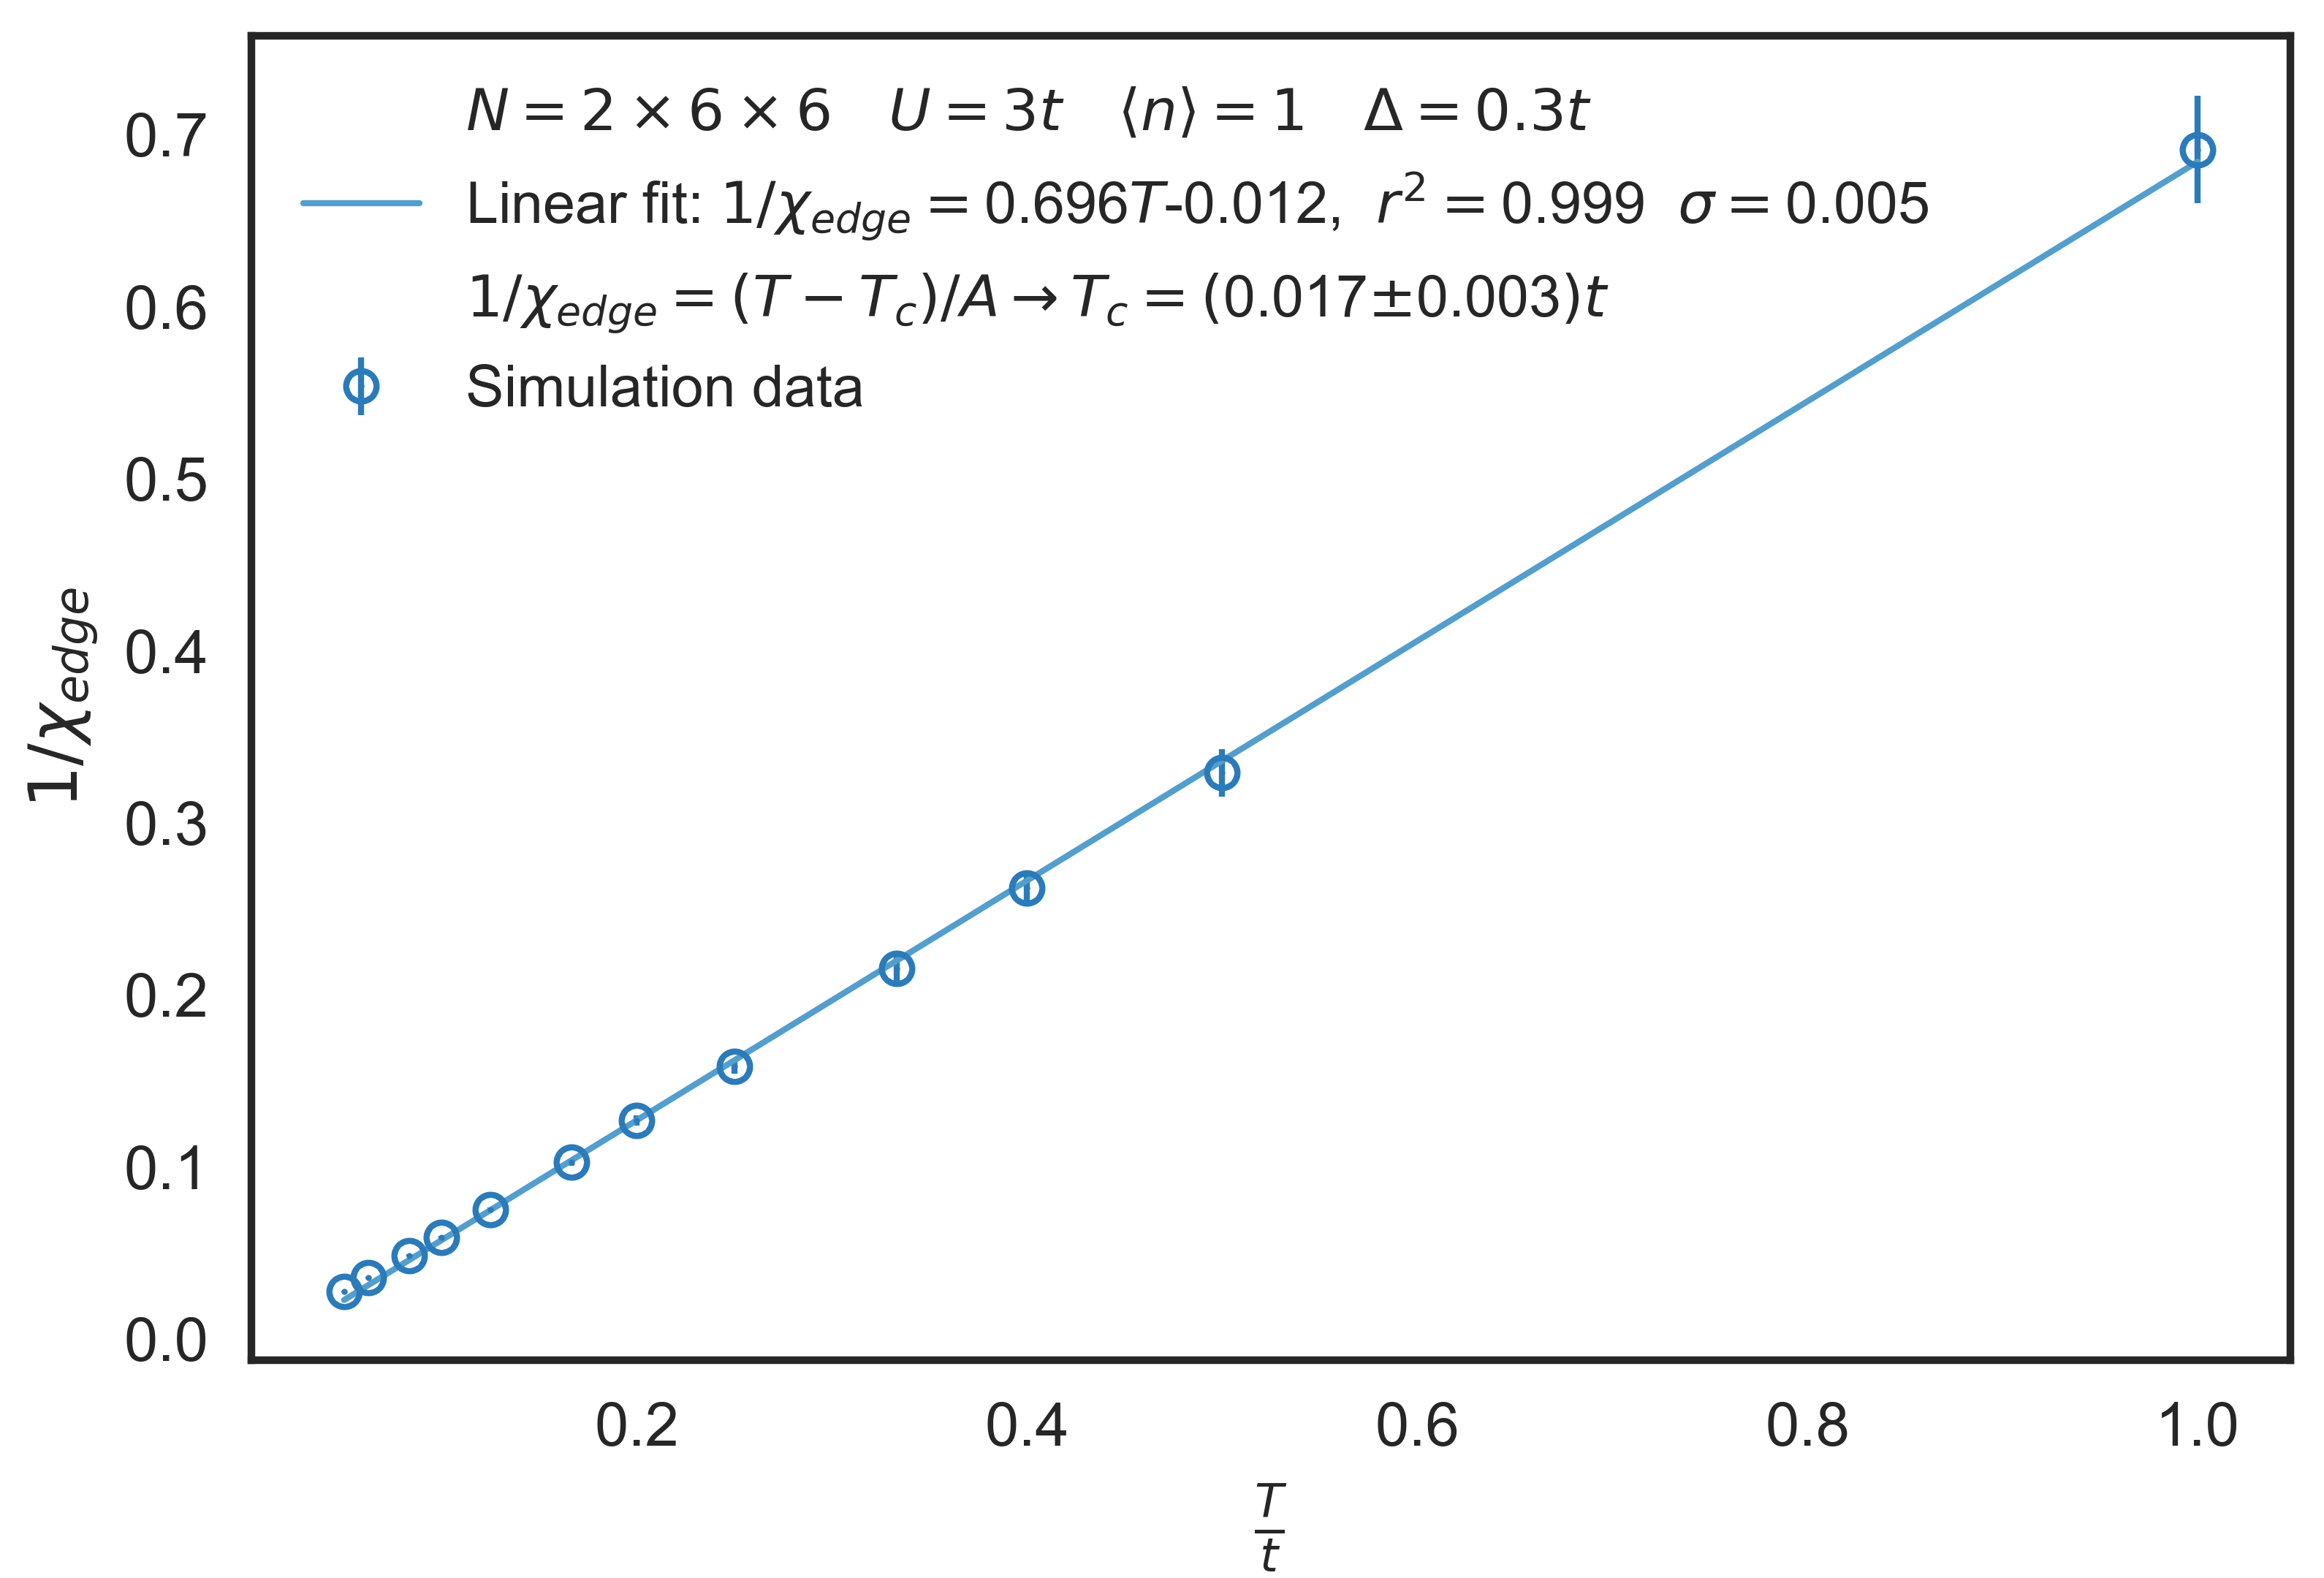
\includegraphics[width=6cm]{images/fityang2017.png}
  \caption{Comparison with \texttt{QUEST}}
  \label{fig:blade_flow_pressure}
\end{figure}
\begin{figure}[H]
  \centering
  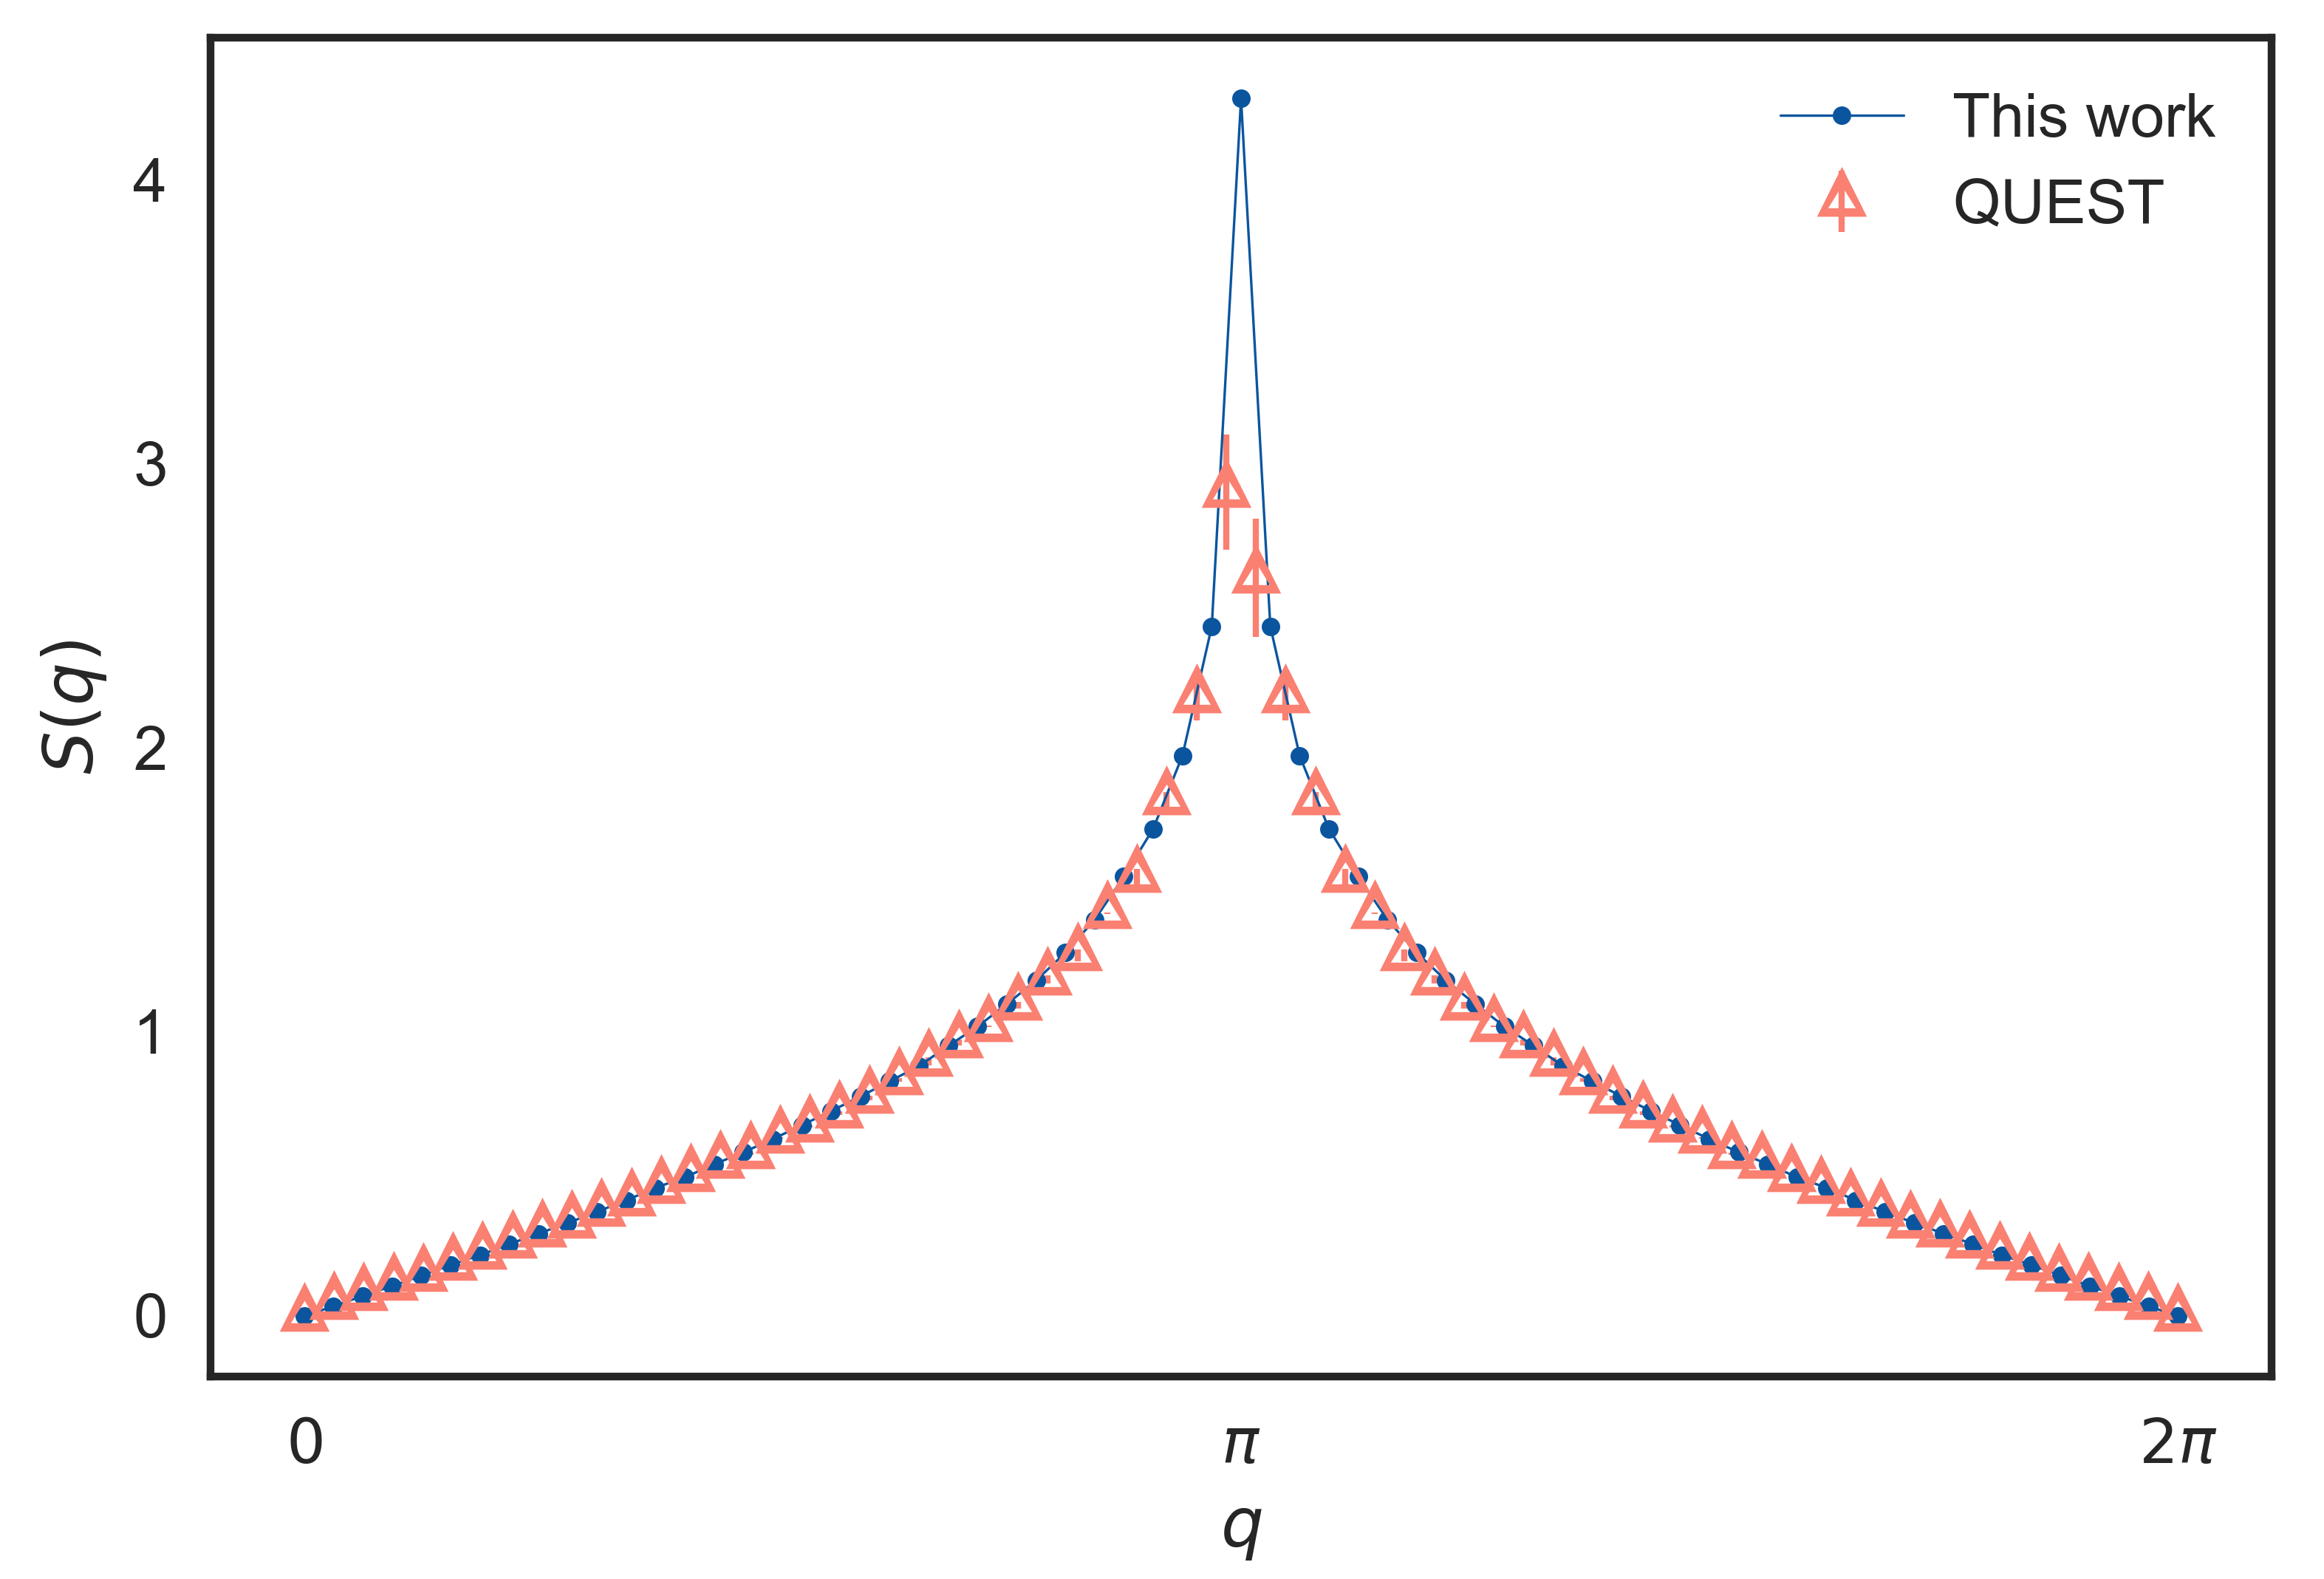
\includegraphics[width=6cm]{images/s_compare.png}
  \caption{Comparison with \texttt{QUEST}}
  \label{fig:blade_flow_pressure}
\end{figure}


%%%%%%%%%%%%%%%%%%%%%%%%%%%%%%%%%%%%%%%%%%%%%%%%%%%%%%%%%%%%%%%%%%%%%%
\subsection{Stabilization}

\begin{figure}[H]
  \centering
  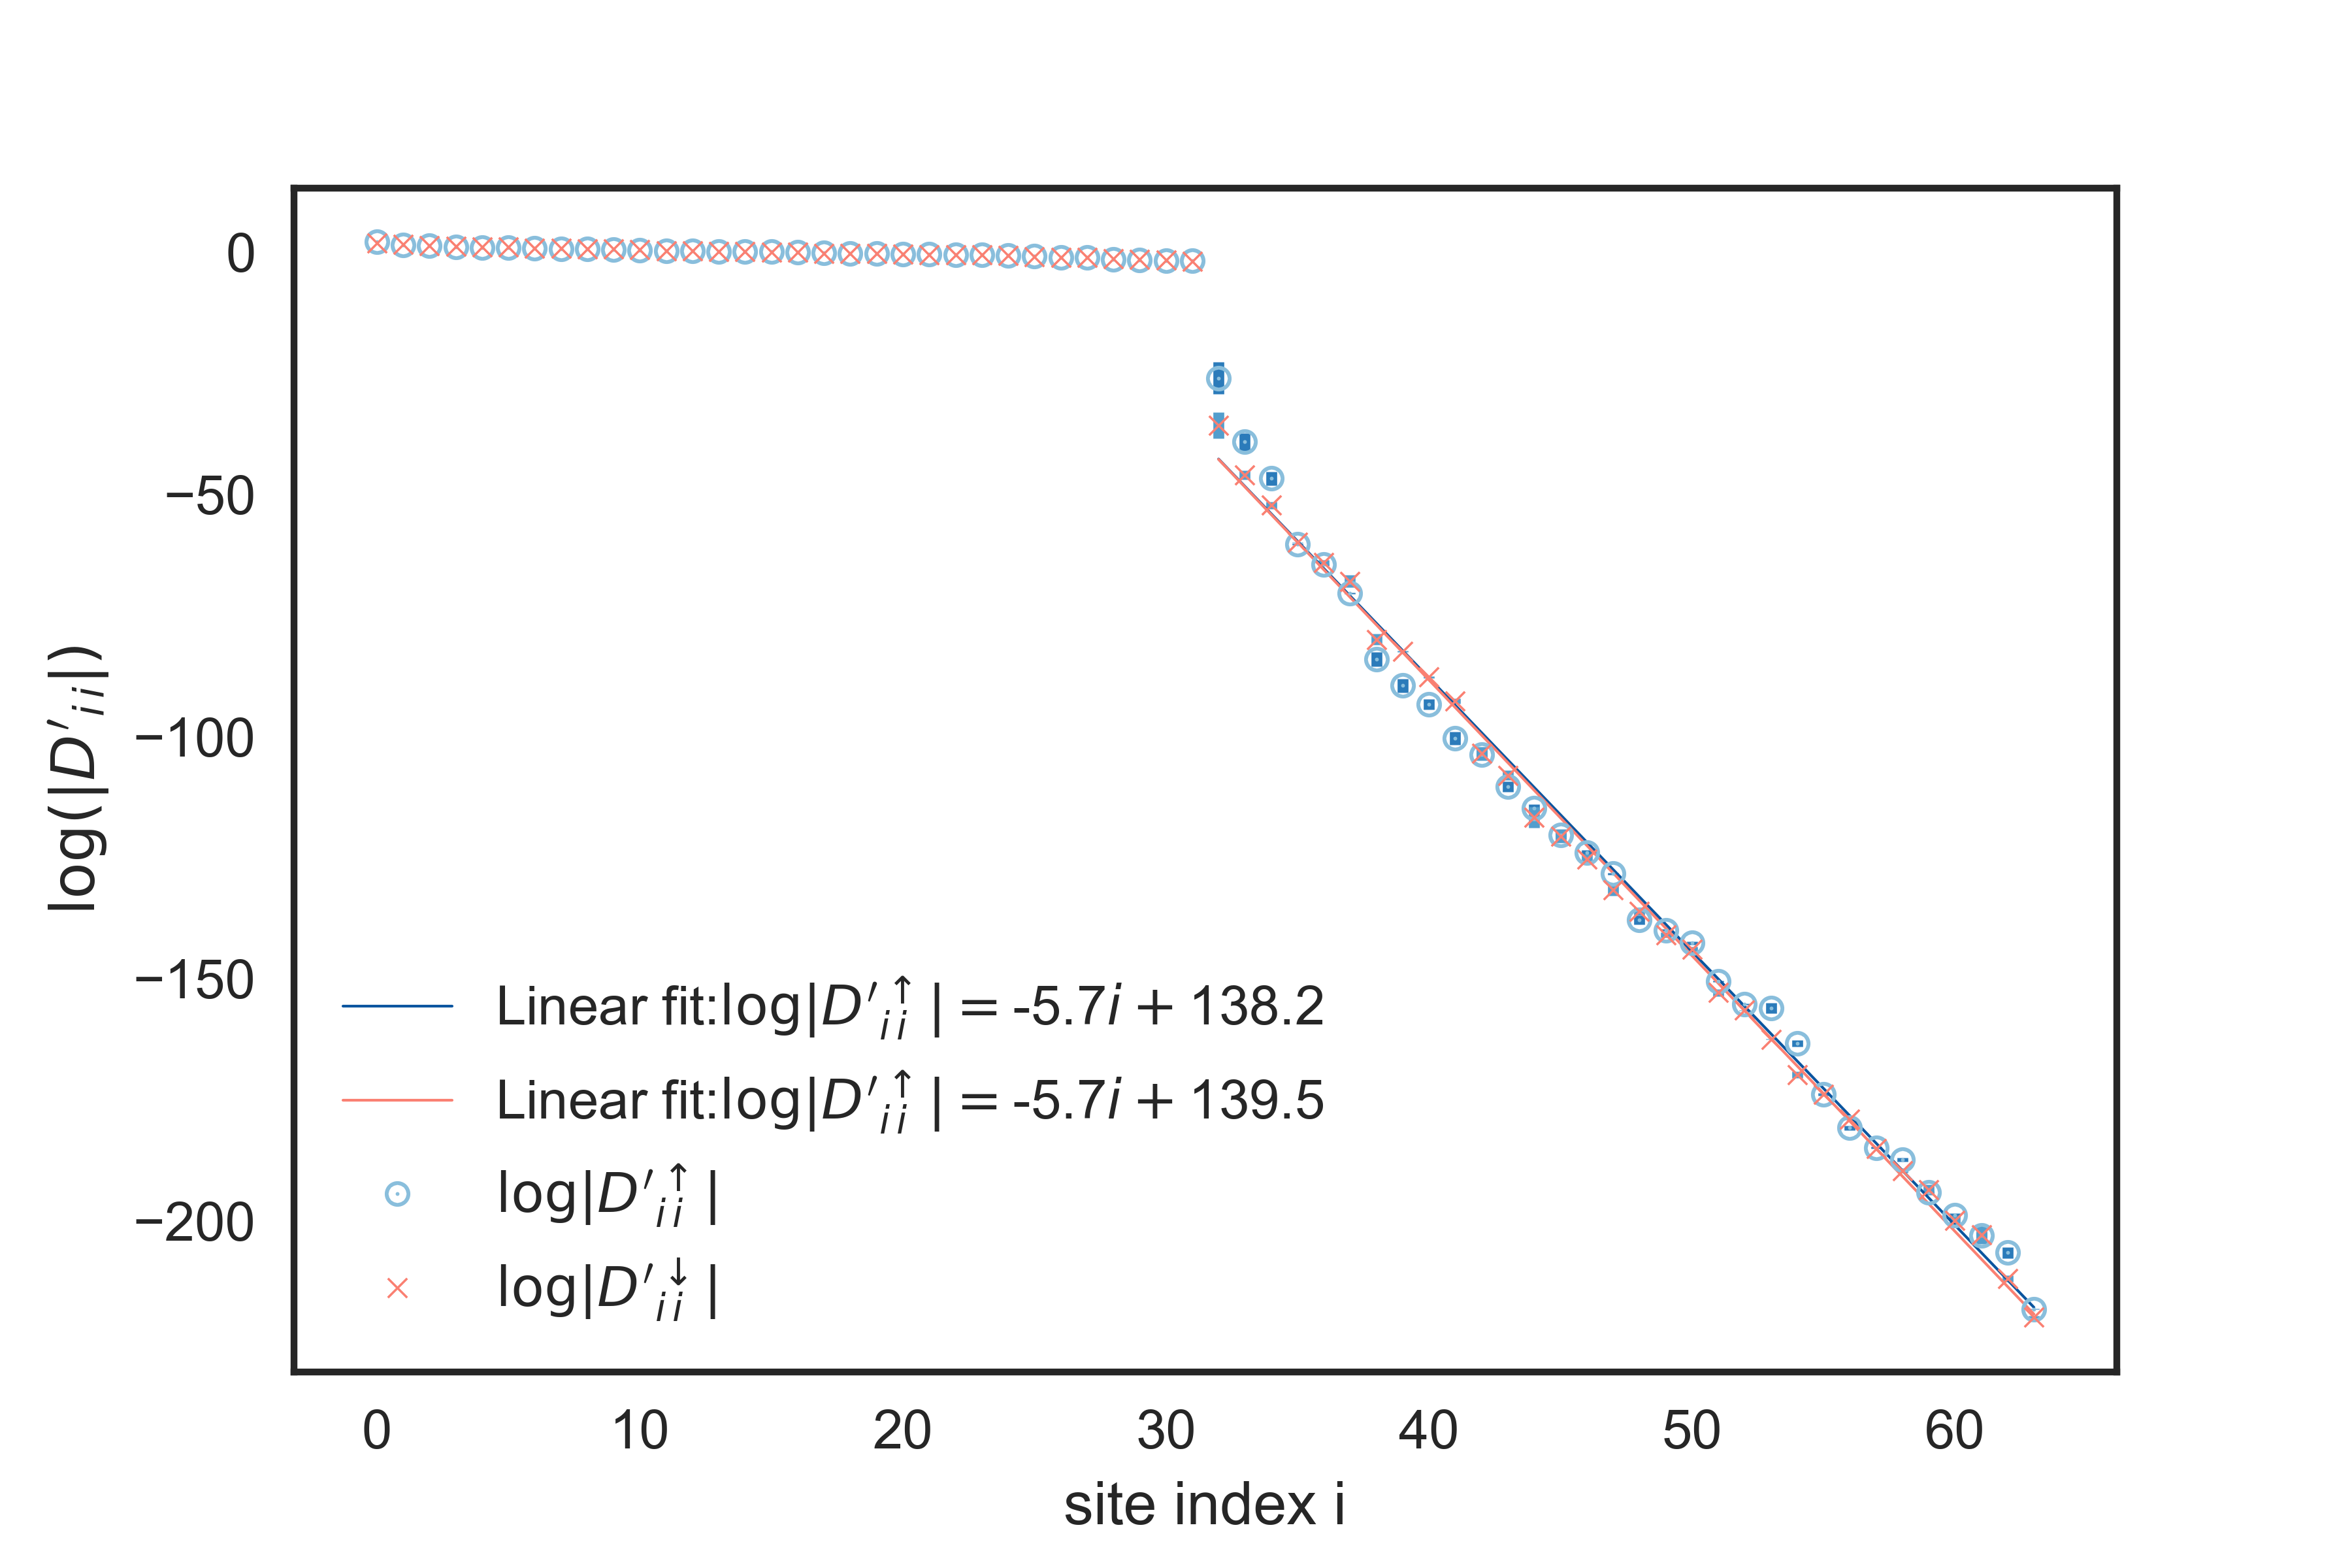
\includegraphics[width=6cm]{images/OrdersOfMagnitude_N=64sites.png}
  \caption{Comparison with \texttt{QUEST}}
  \label{fig:blade_flow_pressure}
\end{figure}



